%%%% début de la page
\teteSndMouv

%%
\nomPrenomClasse


%%%% titre
\numeroActivite{4}
\titreActivite{Principe des actions réciproques}


%%%% evaluation
\pasCorrection{
\vspace*{-8pt}
\begin{tableauCompetences}
  %
  \centering ANA/RAI &
  Analyser les forces qui s'exercent sur un système.
  & & & & \\
  %
  \centering REA &
  Schématiser une situation.
  & & & & \\
  %
  \centering COM &
  Travailler en groupe.
  & & & &
\end{tableauCompetences}
}


%%%% objectifs
\begin{objectifs}
  \item Analyser et schématiser un système en mouvement
  \item Utiliser le principe d'inertie
  \item Comprendre le principe des actions réciproques
\end{objectifs}


%%%%
\begin{doc}{Forces qui se compensent}{doc:A4_forces_compensent}
  \begin{importants}
    On dit que les forces exercées sur un système \important{se compensent}, si leur somme vectorielle est nulle (égale à $\vv{0}$ le vecteur de norme nulle).
    
    \begin{wrapfigure}{r}{0.4\linewidth}
      \vspace*{-40pt}
      \begin{center}
        \begin{tikzpicture}
          % système 
          \tkzCercle{0}{0}{gray!50!white}{20}
          \tkzPointLabel{0}{0}{$A$}
          % forces
          \tkzVecteur(0)[-1.7](0)[-0.75]{$\vv{F}_1$}[left]
          \tkzVecteur(0)[1.7] (0)[0.75] {$\vv{F}_2$}[right]
        \end{tikzpicture}
      
        $\vv{F}_1 + \vv{F}_2 = \vv{0}$, les forces exercée sur le système $A$ se compensent.
      \end{center}
    \end{wrapfigure}
    
    La somme de deux vecteurs est nulle s'ils ont
    
    \begin{listePoints}
      \item \important{même point d'application},
      \item \important{même direction},
      \item \important{même norme},
      \item mais des \important{sens opposés}.
    \end{listePoints}
  \end{importants}
\end{doc}


%%%%
\begin{doc}{Ballon lancé depuis un skateboard}{doc:A4_ballon}
  \begin{flushright}
    \vspace*{-18pt}
    \qrcode{https://youtu.be/Kf0bBxmNeec?t=99}
  \end{flushright}
  \begin{multicols}{3}
    \centering
    \image{0.9}{images/mecanique/lancer_balle_reciproque_1.jpg}
    
    Avant le lancer
    
    \image{0.9}{images/mecanique/lancer_balle_reciproque_2.jpg}

    Pendant le lancer
    
    \image{0.9}{images/mecanique/lancer_balle_reciproque_3.jpg}

    Après le lancer
  \end{multicols}
\end{doc}


%%%
\problematique{Quelle est la force qui met en mouvement la personne sur le skateboard ?}

\numeroQuestion
Étudier le mouvement du système $A$ \og personne sur le skateboard \fg\; et du système $B$ \og ballon \fg\; avant, pendant et après le lancer du ballon.

\numeroQuestion
Décrire les propriétés de la force qui met en mouvement le système $A$.

\fleche Vous Détaillerez soigneusement les étapes de vos raisonnements par écrits sur un compte-rendu complet, compréhensible par un-e élève qui n'aurait pas vu la vidéo.

%\feuilleBlanche